\documentclass[a4paper]{article}
\usepackage{fontspec}
\setmainfont[Ligatures=TeX]{CMU Serif}
\usepackage{WUSTReport}
\usepackage{amsmath}
\usepackage{amssymb}
\usepackage[russian,polish,main=english]{babel}
\usepackage{indentfirst}
\usepackage{natbib}
\usepackage{listings}
\usepackage{matlab-prettifier}
\usepackage{systeme}
\usepackage{todonotes}

\title{Numerical Methods and Optimization Report 2:
  Eigenproblems}
\author{Kinga Otczyk 268473\\Sergiusz Warga 230757}
\date{2025-03-28}
\reporttutor{dr hab. inż. Rafał Zdunek}
\reportgroup{Friday 13:15}

\begin{document}

\maketitle
\tableofcontents
\pagebreak

\section{Problems}
\input{problems/problem_1}
\subsection{Problem 2}%
\label{sec:problem_2}
Solve the following system of linear equations using the selected iterative solvers:
\begin{equation*}
  \systeme{x_1+x_2+x_3=1,x_1+x_2+2x_3=2,x_1+2x_2+2x_3=1}
\end{equation*}
Compare and discuss the computational costs with respect to convergence rates.
Start the iterations from $\matr{x}^{(0)}=\matr{0}$.
%%%%%%%%%%%%%%%%%%%%%%%%%%%%%%%%%%%%%%%%%%%%%%%%%%%%%%%%%%%%%%%%%%%%%%%%%%%%%%%
\subsubsection*{Mathematics}
%%%%%%%%%%%%%%%%%%%%%%%%%%%%%%%%%%%%%%%%%%%%%%%%%%%%%%%%%%%%%%%%%%%%%%%%%%%%%%%
First step that was taken before creating plots, convergence of methods has been checked.
\begin{itemize}
  \item Jacobi \\
  Calculated eigenvalues for this method are 
  \begin{equation*}
    \begin{bmatrix}
      0 \\
      0.5000 \\
      2.0000
    \end{bmatrix}
  \end{equation*}
  Calculated spectral radius for Jacobi method gives $\rho \approx 2$ which disqualifies function from further use.
  \item Gauss-Seidel \\ 
  Eigenvalues for calculating spectral radius are 
  \begin{equation*}
    \begin{bmatrix}
      -2.1091 \\
      0.6498 \\
      1.4593
    \end{bmatrix}
  \end{equation*}
  Resulting in spectral radus $ \rho = 2.1091 $ which doesn't meet the criteria. 
  \item SOR \\
  Optimal $\omega$ relaxation factor wasn't able to be computed.
  Iterative approach for solving this problem didn't find any solution that would get spectral radius within convergence range.
  \item Landweber \\
  First step of calculations would be obtaining resulting matrix of operation $\matr{A}^TA$ for eigenvalue decomposition
  \begin{equation*}
    \matr{A}^TA = 
    \begin{bmatrix}
      1 & 1 & 1 \\
      1 & 2 & 2 \\
      1 & 1 & 2
      \end{bmatrix} * 
      \begin{bmatrix}
        1 & 1 & 1 \\
        1 & 2 & 1 \\
        1 & 2 & 2
      \end{bmatrix} = 
      \begin{bmatrix}
          3 & 5 & 4 \\
          5 & 9 & 7 \\
          4 & 7 & 6
      \end{bmatrix}
  \end{equation*}
  Next step would be obtaining eigenvalues from calculated matrix 
  \begin{equation*}
    \left|\begin{matrix}
      -\lambda+3 & 5 & 4 \\
      5 & -\lambda+9 & 7 \\
      4 & 7 & -\lambda+6
      \end{matrix}=\right|
      = -\lambda^3 + 18\lambda^2 - 9\lambda + 1
  \end{equation*}
  calculated eigenvalues are: 
  \begin{multicols}{3}
    \begin{itemize}
      \item[$\circ$] $\lambda_1 \approx 0.1652 $
      \par
      \item[$\circ$] $\lambda_2 \approx 0.3462 $
      \par
      \item[$\circ$] $\lambda_3 \approx 17.4887 $
    \end{itemize}
  \end{multicols}
  With maximal value determined being $\lambda_3 \approx 17.4887$ we can calculate convergence criteria 
  \begin{equation*}
    2 * |\lambda_{max}(\matr{A}^T\matr{A})|^{-1} = 2 * 17.4887^{-1} \approx 0.1144
  \end{equation*}
  This results in range of converging $\alpha$ values as:
  \begin{equation*}
    0 < \alpha < 0.1144
  \end{equation*}
\end{itemize}

%%%%%%%%%%%%%%%%%%%%%%%%%%%%%%%%%%%%%%%%%%%%%%%%%%%%%%%%%%%%%%%%%%%%%%%%%%%%%%%
\subsubsection*{Solution}
%%%%%%%%%%%%%%%%%%%%%%%%%%%%%%%%%%%%%%%%%%%%%%%%%%%%%%%%%%%%%%%%%%%%%%%%%%%%%%%
Exact solution for this problem is 
\begin{equation*}
  x =
  \begin{bmatrix}
    1 \\
    -1 \\
    1
  \end{bmatrix}
\end{equation*} 
Because of calculated spectral radii of Jacobi, Gauss-Seidel and SOR methods weren't fulfilling the condition $\rho < 1$ these methods couldn't be used in this problem.
For Landweber solution we used $\alpha$ with value of $0.0572$.
\lstinputlisting[linerange={1-10},style=Matlab-editor]{problems/Problem_2.m}
Executing the script results in output:
\lstinputlisting[linerange={11-37},style=Matlab-editor]{problems/Problem_2.m}
\begin{table}[H]
  \centering
  \caption{Calculated results using MATLAB}
  \label{tab:my-table}
  \begin{tabular}{|l|l|l|}
  \hline
  Method               & Landweber                     & Kaczmarz                      \\ \hline
  x\_1                 & 1.0000                        & 1.0000                        \\ \hline
  x\_2                 & -1.0000                       & -1.0000                       \\ \hline
  x\_3                 & 1.0000                        & 1.0000                        \\ \hline
  iterations           & 1046                          & 146                           \\ \hline
  time elapsed {[}s{]} & 2.48 * 10\textasciicircum{}-3 & 8.97 * 10\textasciicircum{}-5 \\ \hline
  \end{tabular}
  \end{table}

  \begin{figure}[H]
    \centering
    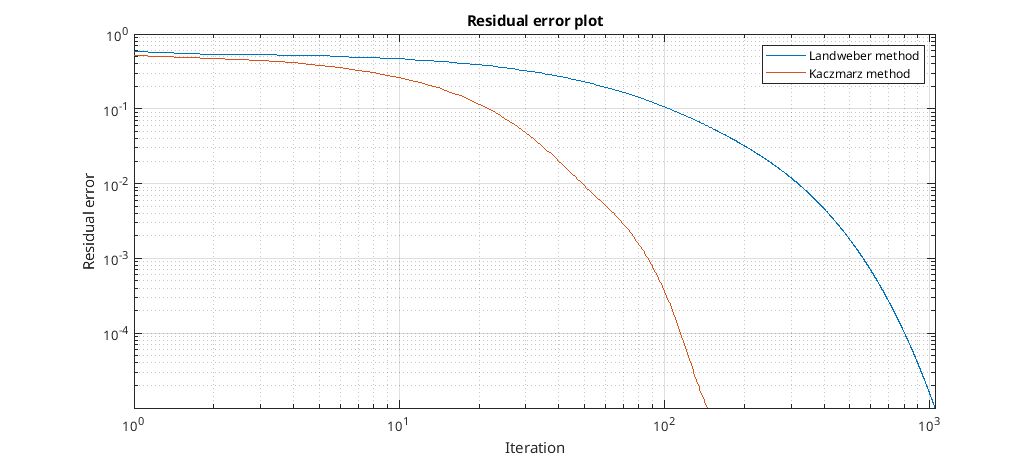
\includegraphics[width=1\textwidth]{images/Residuals_Problem2.png}
    \caption{Residuals of Kaczmarz and Landweber methods}
\end{figure}
\begin{figure}[H]
  \centering
  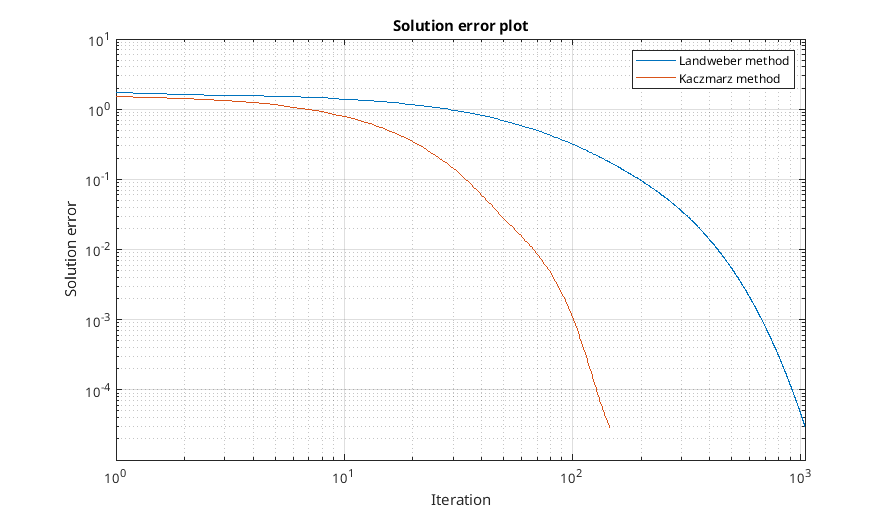
\includegraphics[width=1\textwidth]{images/Solution_Problem2.png}
  \caption{Solution errors of Kaczmarz and Landweber methods}
\end{figure}

\input{problems/problem_7}
\subsection{Problem~11}%
\label{problem:11}

Digitalize a picture into a 640 x 400 (standard VGA) matrix of greyscale pixels, where the value of each pixel is a number $x: 0\leq{}x\leq1$; with black corresponding to $x=0$ and white to $x=1$.
Compute the SVD of this image matrix and display various approximations using 10; 20 and 40 of the singular values and vector pairs.
Do any of these give a good visual approximation of the image?
If not, find a minimal number that works.


\subsubsection*{Solution}
\lstinputlisting[style=Matlab-editor, breaklines=false]{problems/problem_11.m}
\subsection*{The results}
Independent variable was the number of singular values and vector pairs (10, 20, 40, 60, 80, 100). The results are as follows:
\begin{figure}[h]
    \centering
    
\includegraphics[width=0.5\linewidth]{figs/student_rat.png}
    \caption{Original}
    \label{fig:orginal}
\end{figure}
\begin{figure}[h]
    \centering
    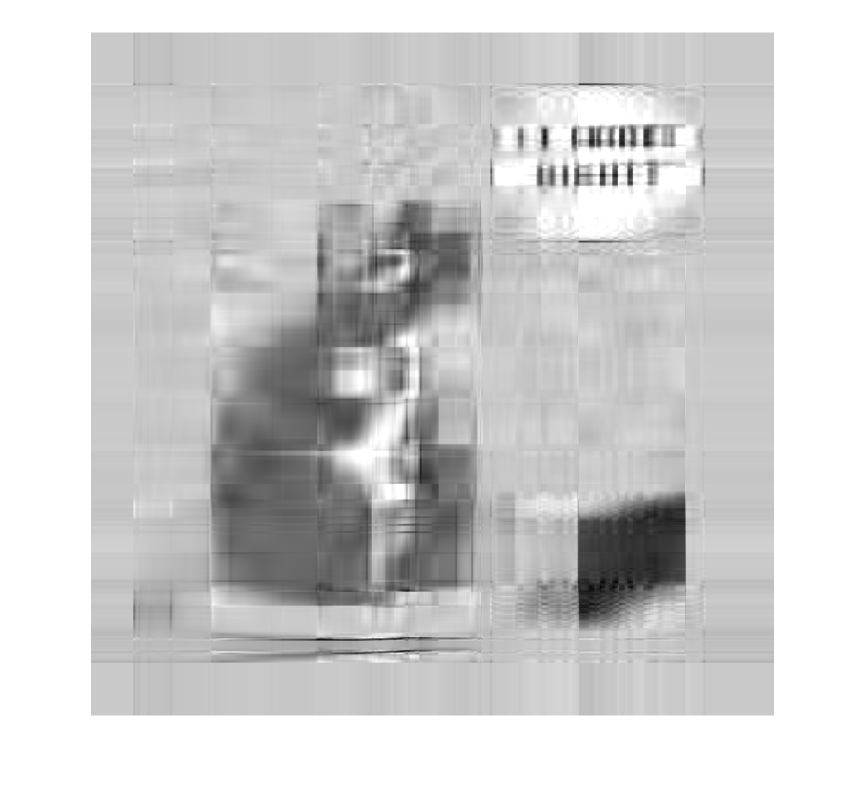
\includegraphics[width=0.5\linewidth]{figs/10_s_v.png}
    \caption{Image output using 10 singular values}
    \label{fig:10_s}
\end{figure}
\begin{figure}[h]
    \centering
    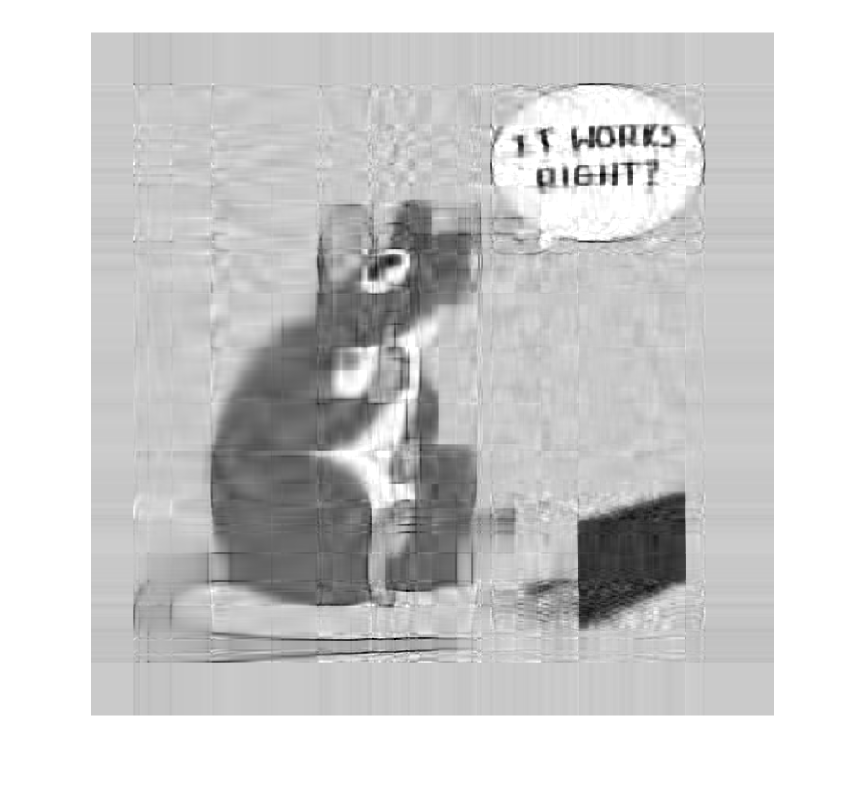
\includegraphics[width=0.5\linewidth]{figs/20_s_v.png}
    \caption{Image output using 20 singular values}
    \label{fig:20_s}
\end{figure}
\begin{figure}[h]
    \centering
    
\includegraphics[width=0.5\linewidth]{figs/40_s_v.png}
    \caption{Image output using 40 singular values}
    \label{fig:40_s}
\end{figure}
\begin{figure}[h]
    \centering
    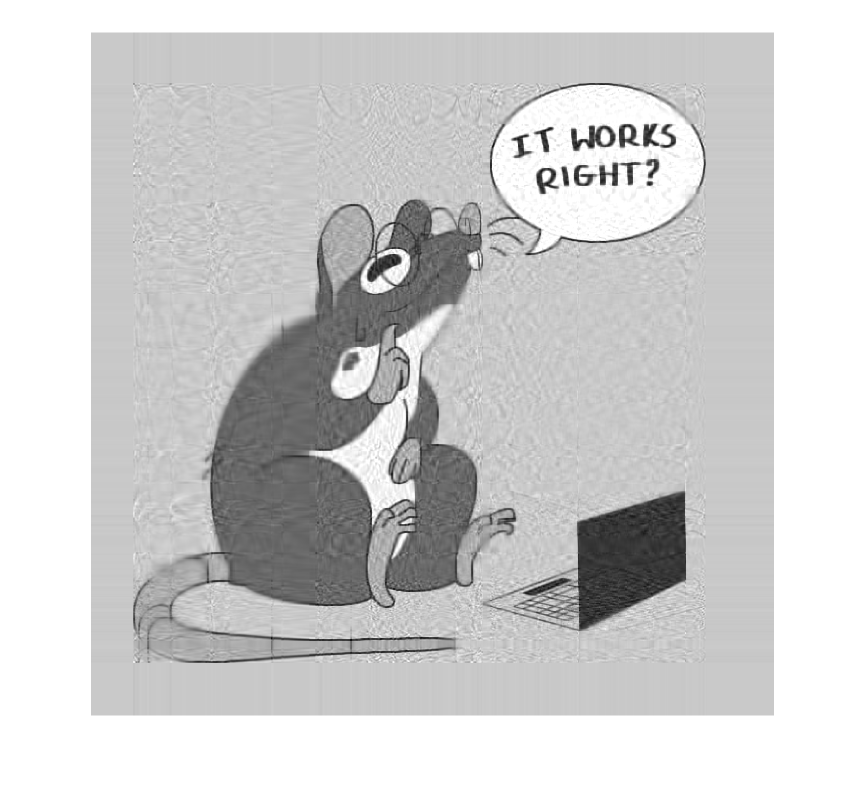
\includegraphics[width=0.5\linewidth]{figs/60_s_v.png}
    \caption{Image output using 60 singular values}
    \label{fig:60_s}
\end{figure}
\begin{figure}[h]
    \centering
    
\includegraphics[width=0.5\linewidth]{figs/80_s_v.png}
    \caption{Image output using 80 singular values}
    \label{fig:80_s}
\end{figure}

As it was observed, 80 seems to be a minimum number of singular values needed
to obtain satisfying results. The image is clear and relatively similar to the original
one:
\begin{figure}
    \centering
    
\includegraphics[width=0.5\linewidth]{figs/100_s_v.png}
    \caption{Image output using 100 singular values}
    \label{fig:100_s}
\end{figure}


\clearpage

\section{Algorithms}
\subsection{Gershgorin disks}%
\label{algorithm:gershgorin}
\lstinputlisting[style=Matlab-editor, breaklines=false]{algorithms/Gershgorin.m}
\subsection{Scaled power algorithm}
\lstinputlisting[style=Matlab-editor, breaklines=false]{algorithms/scaled_power.m}
\subsection{Shift inverse power algorithm}
\lstinputlisting[style=Matlab-editor, breaklines=false]{algorithms/inverse_power.m}

%%%%%%%%%%%%%%%%%%%
%% BIBLIOGRAPHY %%%
%%%%%%%%%%%%%%%%%%%

\clearpage

\nocite{Meyer, GoluVanl96, Zdunek}
\bibliographystyle{alpha}
\bibliography{bibliography}

\end{document}
